\chapter{متعددات الزخم الزاوي، والحركة الشعاعية، وسُلَّم المهتز}

\section{الاعتماد الزاوي للدالة الموجية}

للجسيم في مجال قوة مركزية موضع شعاعي وإحداثيان زاويان. في الوصف الكلاسيكي، يكون \begin{equation}
\mathbf L=\mathbf r\times\mathbf p
\end{equation} محفوظًا بوصفه متجهًا. ويحدِّد اتجاهه مستوى المدار، مع أن المدار ليس بالضرورة دائريًا.

في ميكانيكا الكم يوصف الجسيم بـ \begin{equation}
\Psi=\Psi(r,\theta,\phi),
\end{equation} ويتعلق الزخم الزاوي باعتماد هذه الدالة الموجية على الزوايا.

في بعدين لا توجد إلا مركبة واحدة للزخم الزاوي، هي مولِّد الدورانات حول المحور العمودي على المستوى: \begin{equation}
L_z=-i\hbar\frac{\partial}{\partial\theta}.
\end{equation} وتحقق دالة ذاتية ذات قيمة ذاتية \(\hbar\ell\) العلاقة \begin{equation}
-i\hbar\frac{\partial}{\partial\theta}\psi(r,\theta)
=\hbar\ell\,\psi(r,\theta).
\end{equation} والإحداثي \(r\) لا يتدخل في هذه المعادلة. ويكون حلها على الصورة \begin{equation}
\psi(r,\theta)=\chi(r)e^{i\ell\theta}.
\end{equation} وبالنسبة إلى دالة موجية مدارية اعتيادية أحادية القيمة، فإن الرجوع إلى النقطة نفسها بعد \(\theta\to\theta+2\pi\) يقتضي أن يكون \(\ell\) عددًا صحيحًا. وقد يؤثر العامل الشعاعي \(\chi(r)\) في الطاقة، لكنه لا يؤثر في هذه القيمة الذاتية للزخم الزاوي.

أما النظير ثلاثي الأبعاد فيفصل الاعتماد الشعاعي عن الدوال المعرفة على الكرة: \begin{equation}
\Psi(r,\theta,\phi)=R(r)Y_{\ell m}(\theta,\phi).
\end{equation} والدوال \(Y_{\ell m}\) هي التوافقيات الكروية. ولن نحتاج هنا إلى صيغها الصريحة. تؤثر الدورانات في العامل الزاوي، بينما تُترك الدالة الشعاعية كما هي.

\section{متعددات الزخم الزاوي المنتهية}

تُحقِّق مركبات الزخم الزاوي العلاقة \begin{equation}
\begin{aligned}
[L_x,L_y]&=i\hbar L_z,\\
[L_y,L_z]&=i\hbar L_x,\\
[L_z,L_x]&=i\hbar L_y.
\end{aligned}
\end{equation} اختر حالات ذاتية لـ \(L_z\)، \begin{equation}
L_z|\ell,m\rangle=\hbar m\,|\ell,m\rangle,
\end{equation} وعرِّف \begin{equation}
L_\pm=L_x\pm iL_y.
\end{equation} فتؤدي المبدِّلات \begin{equation}
[L_z,L_\pm]=\pm\hbar L_\pm
\end{equation} إلى \begin{align}
L_z\bigl(L_\pm|\ell,m\rangle\bigr)
&=\bigl(L_\pm L_z+[L_z,L_\pm]\bigr)|\ell,m\rangle \\
&=\hbar(m\pm1)L_\pm|\ell,m\rangle.
\end{align} وبالتالي يرفع \(L_+\) القيمة \(m\) بمقدار واحد، ويخفضها \(L_-\) بمقدار واحد، ما لم ينعدم المتجه الناتج.

في المتعددة المنتهية توجد حالة عليا وحالة دنيا: \begin{equation}
L_+|\ell,\ell\rangle=0,
\qquad
L_-|\ell,-\ell\rangle=0.
\end{equation} ويرتبط اتجاها \(+z\) و\(-z\) بدوران، لذا يكون الطيف المنتهي متناظرًا حول الصفر. ومن ثم تكون قيمه \begin{equation}
m=-\ell,-\ell+1,\ldots,\ell-1,\ell,
\end{equation} ويكون عدد الحالات \begin{equation}
2\ell+1.
\end{equation} وبما أن القيم المتجاورة تختلف بمقدار واحد، فيمكن أن تكون القيم الطرفية أعدادًا صحيحة أو أنصاف أعداد صحيحة. وتحقق التوافقيات الكروية المدارية الاعتيادية الحالة الصحيحة؛ كما أن جبر الزخم الزاوي المجرَّد يجيز أيضًا متعددات أنصاف الأعداد الصحيحة.

\begin{classroomqa}\lecturetimestamp{00:16:12}\audiencequestion{هل يمكن أن تحتوي متعددة زخم زاوي على عدد لا نهائي من الحالات؟}\lecturerresponse{يمكن تصور هذا الاحتمال، لكنه لن يكون مطلوبًا هنا. فالزخم الزاوي يرفع الطاقة عمومًا عندما تُثبَّت السمات الأخرى للحالة، لذا فإن حالات الزخم الزاوي اللانهائي ليست ذات صلة عند مناقشة الحالات ذات الطاقة المنتهية.}\end{classroomqa}

\section{القيمة المشتركة لـ \texorpdfstring{\(L^2\)}{مربع L}}

المؤثر الذي يقيس مربع مقدار الزخم الزاوي هو \begin{equation}
L^2=L_x^2+L_y^2+L_z^2.
\end{equation} والجداء المرتب لمؤثري السُّلَّم هو \begin{align}
L_-L_+
&=(L_x-iL_y)(L_x+iL_y) \\
&=L_x^2+L_y^2+i[L_x,L_y] \\
&=L_x^2+L_y^2-\hbar L_z.
\end{align} وعليه، \begin{equation}
L^2=L_z^2+\hbar L_z+L_-L_+.
\end{equation} طبِّق هذه المتطابقة على الحالة العليا. وبما أن \(L_+|\ell,\ell\rangle=0\)، فإن \begin{align}
L^2|\ell,\ell\rangle
&=\left(L_z^2+\hbar L_z+L_-L_+\right)|\ell,\ell\rangle \\
&=\hbar^2\left(\ell^2+\ell\right)|\ell,\ell\rangle,
\end{align} ومن ثم \begin{equation}
L^2|\ell,\ell\rangle
=\hbar^2\ell(\ell+1)|\ell,\ell\rangle.
\end{equation} ومربع المقدار ليس \(\hbar^2\ell^2\). والحد الإضافي هو نتيجة لعدم تبديلية مركبات الزخم الزاوي.

وتخص هذه القيمة نفسها كل حالة في المتعددة، لا الحالة العليا وحدها.

\begin{classroomqa}\lecturetimestamp{00:26:08}\audiencequestion{ما الذي يبرهنه التمرين بالضبط لإظهار أن الحالات الأخرى لها القيمة نفسها لـ \(L^2\)؟}\lecturerresponse{أثبت أن \(L^2\) يبادل كل مركبة من مركبات الزخم الزاوي، ومن ثم يبادل \(L_-\). ثم مرِّر \(L^2\) عبر \(L_-\): فإذا كانت للحالة العليا القيمة الذاتية \(\hbar^2\ell(\ell+1)\)، فإن الحالة التالية نزولًا لها القيمة الذاتية نفسها. ويؤدي تكرار الحجة إلى حمل هذه القيمة على امتداد السُّلَّم كله.}\end{classroomqa}

وبالفعل، \begin{equation}
[L^2,L_i]=0,
\qquad i=x,y,z,
\end{equation} ومن ثم \begin{equation}
[L^2,L_\pm]=0.
\end{equation} فعلى سبيل المثال، \begin{align}
L^2\bigl(L_-|\ell,\ell\rangle\bigr)
&=L_-L^2|\ell,\ell\rangle \\
&=\hbar^2\ell(\ell+1)L_-|\ell,\ell\rangle.
\end{align} ومواصلة النزول تعطي \begin{equation}
L^2|\ell,m\rangle
=\hbar^2\ell(\ell+1)|\ell,m\rangle
\end{equation} لكل \(m=-\ell,\ldots,\ell\).

ويعطي الترتيب المعاكس تحليلًا مكافئًا: \begin{align}
L_+L_-
&=(L_x+iL_y)(L_x-iL_y) \\
&=L_x^2+L_y^2-i[L_x,L_y] \\
&=L_x^2+L_y^2+\hbar L_z,
\end{align} ومن ثم \begin{equation}
L^2=L_z^2-\hbar L_z+L_+L_-.
\end{equation}

\begin{classroomqa}\lecturetimestamp{00:32:05}\audiencequestion{هل يمكن تحليل \(L_x^2+L_y^2\) بالترتيب المعاكس باستخدام \(L_+L_-\)؟}\lecturerresponse{نعم. تنعكس إشارة حد \(L_z\). ومع هذا الترتيب، تُطبَّق المتطابقة على الحالة الدنيا التي يُفنيها \(L_-\)، لا على الحالة العليا. وتنتج القيمة الذاتية نفسها \(\hbar^2\ell(\ell+1)\).}\end{classroomqa}

وعليه فإن التوافقيات الكروية تحقق \begin{align}
L^2Y_{\ell m}
&=\hbar^2\ell(\ell+1)Y_{\ell m}, \\
L_zY_{\ell m}
&=\hbar m\,Y_{\ell m}.
\end{align} ولكل قيمة مدارية \(\ell=0,1,2,\ldots\)، توجد \(2\ell+1\) دالة موسومة بـ \(m=-\ell,\ldots,\ell\).

في حالة جهد مركزي، \begin{equation}
[H,L_i]=0.
\end{equation} وعند تثبيت حالة ذاتية شعاعية للطاقة و\(\ell\)، فإن تغيير \(m\) بواسطة \(L_\pm\) لا يغيِّر الطاقة. لذا فإن كل حالة ذاتية شعاعية من هذا النوع تولِّد متعددة مغناطيسية ذات بُعد \(2\ell+1\).

يظهر سُلَّم الزخم الزاوي المداري الصحيح أدناه.\footnote{أُعيد بناء الشكل من مخطط المتعددة ومتطابقات المؤثرات الظاهرة عند \(00{:}35{:}53\) من فيديو المحاضرة.}

\begin{figure}[htbp]\centering
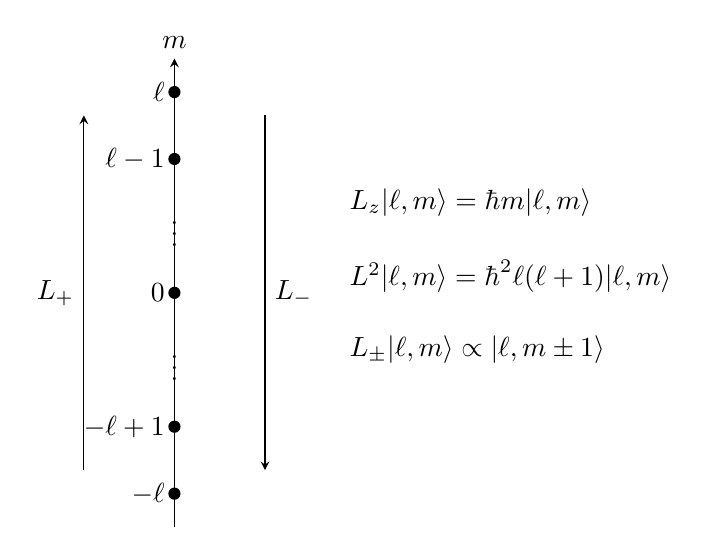
\begin{tikzpicture}[x=1cm,y=0.85cm,>=stealth]
\draw[->] (0,-3.5) -- (0,3.5) node[above] {$m$};

\fill (0,3) circle (2.2pt);
\fill (0,2) circle (2.2pt);
\fill (0,0) circle (2.2pt);
\fill (0,-2) circle (2.2pt);
\fill (0,-3) circle (2.2pt);

\node[left] at (0,3) {$\ell$};
\node[left] at (0,2) {$\ell-1$};
\node[left] at (0,0) {$0$};
\node[left] at (0,-2) {$-\ell+1$};
\node[left] at (0,-3) {$-\ell$};

\node at (0,1) {$\vdots$};
\node at (0,-1) {$\vdots$};

\draw[->] (-1.15,-2.65) -- (-1.15,2.65)
node[midway,left] {$L_+$};
\draw[->] (1.15,2.65) -- (1.15,-2.65)
node[midway,right] {$L_-$};

\node[anchor=west] at (2.1,1.35)
{$L_z|\ell,m\rangle=\hbar m|\ell,m\rangle$};
\node[anchor=west] at (2.1,0.25)
{$L^2|\ell,m\rangle=\hbar^2\ell(\ell+1)|\ell,m\rangle$};
\node[anchor=west] at (2.1,-0.85)
{$L_\pm|\ell,m\rangle\propto|\ell,m\pm1\rangle$};
\end{tikzpicture}\caption{متعددة صحيحة للزخم الزاوي المداري. يغيِّر \(L_+\) و\(L_-\) القيمة \(m\) بمقدار واحد، بينما يبقى \(L^2\) مساويًا لـ \(\hbar^2\ell(\ell+1)\) على امتداد المتعددة.}\lectureframe{00:35:53}\end{figure}

\section{مسألة القوة المركزية}

انظر إلى \begin{equation}
H=\frac{\mathbf p^2}{2m}+V(r),
\end{equation} حيث إن \(V\) يعتمد فقط على البعد عن الأصل. ويقتضي التناظر الدوراني انحفاظ الزخم الزاوي. كلاسيكيًا، يكون لـ \(\mathbf L\) مقدار واتجاه ثابتان، لذا يبقى المدار في مستوى عمودي على \(\mathbf L\). وليس من الضروري أن يكون المدار دائريًا، ولا حتى مغلقًا.

اختر إحداثيات بحيث يكون هذا المستوى المداري الكلاسيكي هو مستوى \(xy\)، وحلّل الزخم إلى مركبتين شعاعية ومماسية: \begin{equation}
\mathbf p^2=p_r^2+p_\theta^2.
\end{equation} وبما أن مقدار الزخم الزاوي هو \begin{equation}
L=r p_\theta,
\end{equation}، فيمكن كتابة المساهمة المماسية على الصورة \begin{equation}
p_\theta^2=\frac{L^2}{r^2}.
\end{equation} ويصبح الهاملتوني \begin{equation}
H=\frac{p_r^2}{2m}+\frac{L^2}{2mr^2}+V(r).
\end{equation} وعند تثبيت \(L\)، فهذه مسألة أحادية البعد في الإحداثي الشعاعي، ذات جهد فعال \begin{equation}
V_{\mathrm{eff}}(r)=\frac{L^2}{2mr^2}+V(r).
\end{equation} ويظهر الهاملتوني الشعاعي على اللوح أدناه.\footnote{إطار المصدر: \texttt{\detokenize{lecture_03_frame_02.png}}، فيديو المحاضرة عند \(00{:}47{:}15\).}

\begin{figure}[htbp]\centering
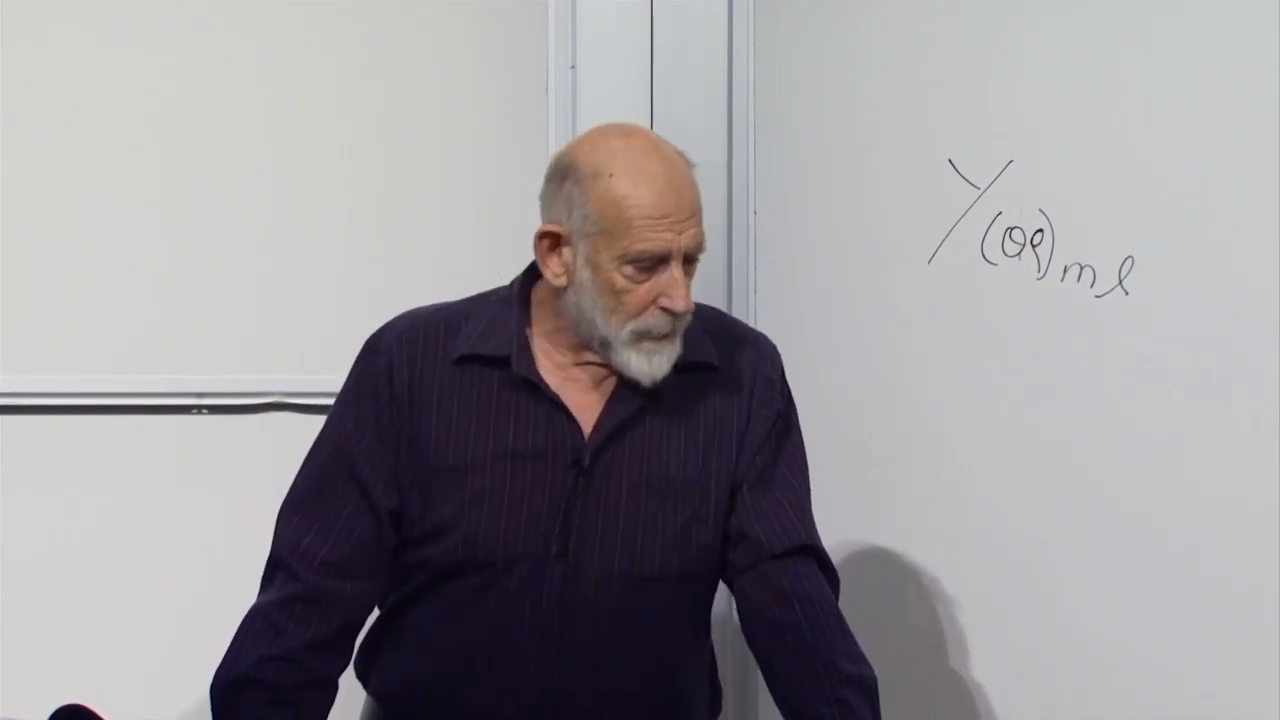
\includegraphics[width=0.9\linewidth]{lecture_03_frame_02.png}\caption{عند تثبيت الزخم الزاوي الكلاسيكي، يحتوي الهاملتوني الشعاعي على طاقة حركة شعاعية، وحد الطرد المركزي \(L^2/(2mr^2)\)، والجهد المركزي \(V(r)\).}\lectureframe{00:47:15}\end{figure}

إن حد \(1/r^2\) هو حاجز الطرد المركزي. فهو يزداد حين يقترب الجسيم من الأصل، ولذلك تتجه القوة المصاحبة إلى الخارج. وبالنسبة إلى تجاذبات شبيهة بكولوم من النوع قيد المناقشة، فإن مسارًا له \(L\neq0\) يلتف حول المركز بدلًا من بلوغه. وعندما يكون \(L=0\)، يغيب هذا الحاجز.

بالنسبة إلى جهد كولوم التجاذبي، \begin{equation}
V(r)=-\frac{\kappa}{r},
\end{equation} يسود حد الطرد المركزي عند القيم الصغيرة لـ \(r\)، بينما يتناقص حد كولوم على نحو أبطأ ويسود عند القيم الكبيرة لـ \(r\). وعندما يكون \(L\neq0\)، يكون لمجموعهما حد أدنى. وتكون الحركة عند هذا الحد الأدنى ذات نصف قطر ثابت، ومن ثم فهي دائرية. أما الحركة المقيدة فوق الحد الأدنى وتحت عتبة الإفلات فتتذبذب بين أصغر نصف قطر وأكبره؛ وفي مسألة كولوم تكون هذه هي الاهتزازات الشعاعية لمدار إهليلجي.

\section{المعادلة الشعاعية المختزلة}

في ميكانيكا الكم يكون الجزء الزاوي من حالة ذات زخم زاوي مداري محدد توافقًا كرويًا. اكتب الحالة المفصولة على الصورة \begin{equation}
\Psi_{n_r\ell m}(r,\theta,\phi)
=\frac{u_{n_r\ell}(r)}{r}\,
Y_{\ell m}(\theta,\phi).
\end{equation} وللمؤثر الزاوي \(L^2\) القيمة الذاتية \begin{equation}
L^2Y_{\ell m}
=\hbar^2\ell(\ell+1)Y_{\ell m}.
\end{equation} ولزوج ثابت \(n_r,\ell\)، اختصر \(u_{n_r\ell}(r)\) إلى \(u(r)\). وتكون المعادلة المتبقية للدالة الشعاعية المختزلة هي \begin{equation}
\begin{aligned}
&-\frac{\hbar^2}{2m}\frac{d^2u}{dr^2}
+\frac{\hbar^2\ell(\ell+1)}{2mr^2}u(r)\\
&\qquad+V(r)u(r)=E_{n_r\ell}\,u(r).
\end{aligned}
\end{equation}

\editorialnote{تستخدم المعادلة الأحادية البعد الخالصة ذات المشتقة الثانية الدالة الشعاعية المختزلة \(u=rR\). وبذلك فإن \(\psi(r)\) في معادلة المحاضرة المعروضة يقابل \(u(r)\)، بينما العامل الشعاعي العادي في \(\Psi=R(r)Y_{\ell m}\) هو \(R=u/r\). ويتجنب هذا الاصطلاح معاملة \(-i\hbar\,d/dr\) بوصفه مؤثر زخم شعاعي هيرميتيًا قائمًا بذاته على فضاء هيلبرت الشعاعي الثلاثي الأبعاد.}

تظهر المعادلة الشعاعية المختزلة على اللوح أدناه.\footnote{إطار المصدر: \texttt{\detokenize{lecture_03_frame_03.png}}، فيديو المحاضرة عند \(00{:}54{:}32\).}

\begin{figure}[htbp]\centering
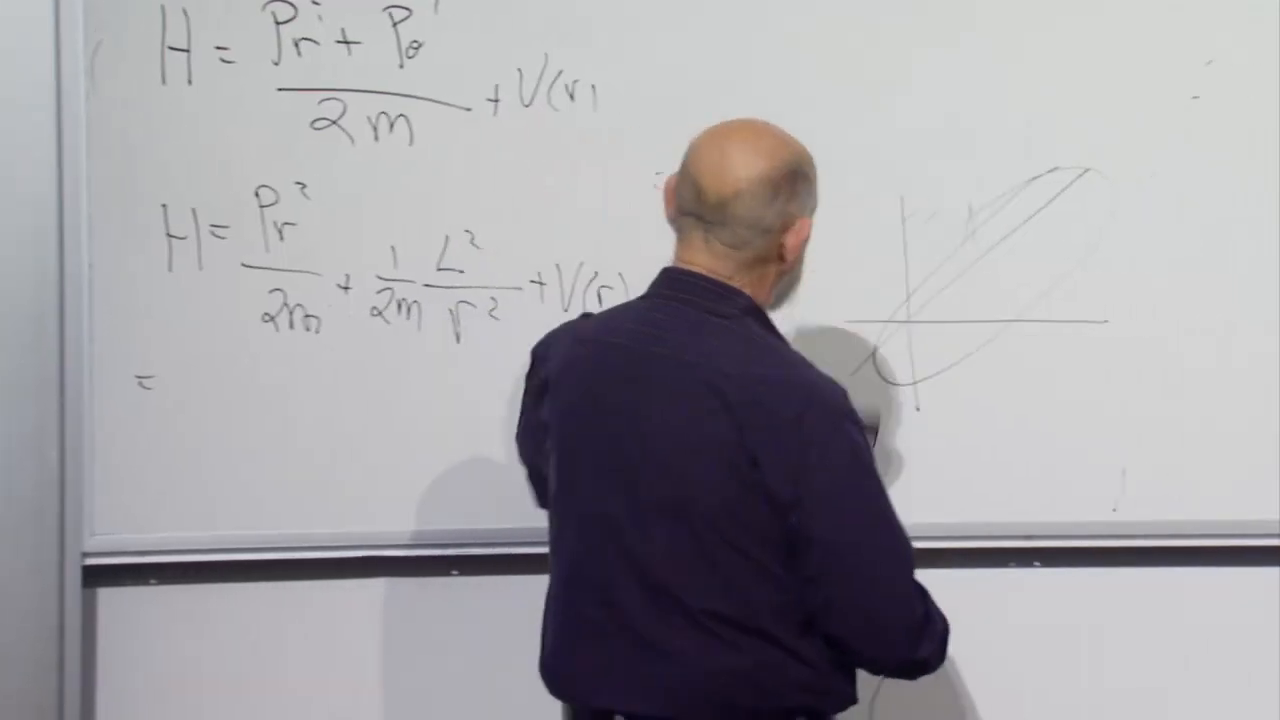
\includegraphics[width=0.9\linewidth]{lecture_03_frame_03.png}\caption{عند تثبيت \(\ell\)، تخضع الدالة الموجية الشعاعية المختزلة لمعادلة Schr\"odinger أحادية البعد مع حد طرد مركزي يتناسب مع \(\ell(\ell+1)/r^2\).}\lectureframe{00:54:32}\end{figure}

لقد اختُزل البنيان الزاوي الثلاثي الأبعاد في المعلمة \(\ell\). ولا يظهر العدد الكمي المغناطيسي \(m\) في المعادلة الشعاعية.

\begin{classroomqa}\lecturetimestamp{00:55:34}\audiencequestion{بالنسبة إلى \(\ell\) معيَّن، هل تمتلك الحالات المغناطيسية \(2\ell+1\) الطاقة نفسها؟}\lecturerresponse{نعم، شريطة تثبيت الحالة الذاتية الشعاعية أيضًا. فلكل \(u_{n_r\ell}\) مختار، تكون لجميع القيم \(m=-\ell,\ldots,\ell\) الطاقة نفسها لأن \(m\) لا يدخل في المعادلة الشعاعية. أما الحالات الذاتية الشعاعية المختلفة عند \(\ell\) نفسه فلها عمومًا طاقات مختلفة.}\end{classroomqa}

\begin{classroomqa}
\lecturetimestamp{00:56:03}
\audiencequestion{لماذا يمكن استبدال \(L^2\) بـ \(\hbar^2\ell(\ell+1)\)، وكيف ترتبط \(\ell\) بالقيم المسموح بها لـ \(m\)؟}
\lecturerresponse{العدد \(\ell\) يميّز متعددية العزم الزاوي، وهو أكبر قيمة فيها لـ \(m\). ولكل حالة في تلك المتعددية القيمة الذاتية نفسها لـ \(L^2\)، وهي \(\hbar^2\ell(\ell+1)\)، ولذلك تُدرج تلك القيمة الذاتية في المعادلة الشعاعية.}
\end{classroomqa}

لا نحتاج إلى الحلول الصريحة بالدوال الخاصة في الاستدلال الحالي. وما يهم هو كيفية تنظيم الحلول.

\section{العقد الشعاعية ومستويات الطاقة}

عند تثبيت \(\ell\)، تكون المعادلة الشعاعية المختزلة مسألة قيم ذاتية عادية أحادية البعد. وتُرتَّب حالاتها المقيدة بحسب عدد العقد الداخلية فيها. فأدنى حالة شعاعية لا تحتوي على أي عقدة داخلية، والتي تليها تحتوي على عقدة واحدة، والتي بعدها تحتوي على عقدتين. وتعني زيادة عدد العقد تغيرًا أسرع في الدالة الموجية؛ والتغير الأسرع يعني زخمًا أكبر، ومن ثم طاقة حركية أكبر.

يحدِّد كل مقدار من \(\ell\) مؤثرًا شعاعيًا مختلفًا لأن الحد النابذ المركزي يتغير مع \(\ell\). ومن ثم فإن \(\ell=0,1,2,\ldots\) تعطي سلاسل شعاعية منفصلة. ويزيح الحد النابذ المركزي الموجب المستويات إلى أعلى مع إضافة العزم الزاوي. وتحمل كل قيمة ذاتية شعاعية عند تثبيت \(\ell\) متعددية مغناطيسية بُعدها
\begin{equation}
2\ell+1.
\end{equation}
والمستويات ذات \(\ell=0\) أحادية، وذات \(\ell=1\) ثلاثية، وذات \(\ell=2\) خماسية. وهذه هي الانحلالات التي يضمنها التناظر الدوراني؛ وقد يجعل تناظر إضافي أيضًا الحالات ذات القيم المختلفة لـ \(\ell\) منحلةً كذلك.

بالنسبة إلى الكمونات من النوع الذري التي تحقق \(V(r)\to0\) عند القيم الكبيرة لـ \(r\)، تؤخذ عتبة الإفلات اصطلاحًا عند \(E=0\). وتشكل حالات الطاقة السالبة الطيف المنفصل المقيد. وعند \(E=0\) وما فوقه نصادف المتصل التشتتي. وتعتمد هذه العبارة على سلوك الكمون عند القيم الكبيرة لـ \(r\)، ولا تنطبق على كمون مركزي حابس.

\section{الانحلال الكولومي الخاص}

للکمون الكولومي الدقيق اللامنسبي اصطفاف إضافي للمستويات. فللحالة الشعاعية الدنيا ذات \(\ell=1\) الطاقة نفسها التي لأول حالة مثارة ذات \(\ell=0\). وتتراصف الحالة التالية ذات \(\ell=1\) مع ثاني حالة مثارة ذات \(\ell=0\)، وتنضم إليهما الحالة الدنيا ذات \(\ell=2\). ويستمر هذا النمط عبر السلاسل الأعلى شعاعيًا وزاويًا.

\begin{classroomqa}
\lecturetimestamp{01:09:57}
\audiencequestion{هل يشير هذا الانحلال الكولومي الإضافي إلى تناظر آخر؟}
\lecturerresponse{نعم. إنه تناظر إضافي غير مألوف للكمون الكولومي الدقيق. فالتغييرات الصغيرة في الكمون تفسد هذا الاصطفاف، ولا نتابع اشتقاقه هنا.}
\end{classroomqa}

وتكون انحلالات الأغلفة المدارية الناتجة
\begin{equation}
1,\qquad 4,\qquad 9,\qquad 16,\qquad \ldots
\end{equation}
قبل إدخال اللف المغزلي للإلكترون.

\begin{classroomqa}
\lecturetimestamp{01:11:46}
\audiencequestion{هل يصف هذا الانحلال الهيدروجين، أم يصف فقط مسألة كولوم المثالية؟}
\lecturerresponse{يحققه الهيدروجين تقريبًا جيدًا جدًا، ولكن ليس على نحو دقيق تمامًا. فالتصحيحات النسبية والحجم المنتهي للنواة يخلّان بالنمط الكولومي المثالي.}
\end{classroomqa}

تعطي النواة النقطية كمونًا دقيقًا من النمط \(1/r\). أما النواة التي تكون شحنتها موزعة على حجم صغير فتولد كمونًا مختلفًا قليلًا عندما ينفذ الإلكترون إلى ذلك الحجم، وحتى هذا الانحراف الصغير يزيل جزءًا من الانحلال الخاص.

وقد أُهمل اللف المغزلي أيضًا. إن إدخال حالتي اللف المغزلي للإلكترون يضاعف عدد الحالات في الأغلفة ليصبح
\begin{equation}
2,\qquad 8,\qquad 18,\qquad 32,\qquad \ldots
\end{equation}
قبل تمييز الانشقاقات الإضافية في معالجة ذرية أكثر اكتمالًا.

\section{إعادة النظر في المعادلة الديكارتية}

المعادلة التي بدأت منها المسألة الشعاعية هي معادلة Schr\"odinger ثلاثية الأبعاد المستقلة عن الزمن
\begin{equation}
\begin{aligned}
-\frac{\hbar^2}{2m}\nabla^2\Psi+V(r)\Psi&=E\Psi,\\
\nabla^2&=\frac{\partial^2}{\partial x^2}
+\frac{\partial^2}{\partial y^2}
+\frac{\partial^2}{\partial z^2},\\
r&=\sqrt{x^2+y^2+z^2}.
\end{aligned}
\end{equation}
ثم ننتقل إلى الإحداثيات الشعاعية والزاوية ونختار حالة ذاتية لـ \(L^2\). وعندئذ يؤدي استبدال \(L^2\) بـ \(\hbar^2\ell(\ell+1)\) إلى اختزال المعادلة التفاضلية الجزئية إلى المعادلة الشعاعية العادية أعلاه.

\begin{classroomqa}
\lecturetimestamp{01:16:42}
\audiencequestion{هل يمكن استخدام الانحرافات عن طيف كولوم المثالي لتحديد حجم النواة؟}
\lecturerresponse{ليس بهذه المقارنة البسيطة. فهناك تصحيحات أخرى أكبر بكثير، ويجب أخذها في الحسبان أولًا. ويُذكر حجم النواة هنا لأنه يعطي مثالًا مباشرًا على انحراف عن كمون كولوم النقطي.}
\end{classroomqa}

\begin{classroomqa}
\lecturetimestamp{01:17:09}
\audiencequestion{ما الفرق الرئيسي بين حدي العزم الزاوي الكلاسيكي والكمومي؟}
\lecturerresponse{كلاسيكيًا، يكون \(L^2\) هو المربع المعتاد لمقدار متجه محفوظ. أما في متعددية مدارية كمومية فقيمته الذاتية هي \(\hbar^2\ell(\ell+1)\)، لا ببساطة \(\hbar^2\ell^2\). ويأتي الحد الإضافي من عدم تبديل مركبات العزم الزاوي.}
\end{classroomqa}

\begin{classroomqa}
\lecturetimestamp{01:17:58}
\audiencequestion{هل للدوال الموجية للحالات المقيدة دعم متراص؟}
\lecturerresponse{لا. فهي تمتد إلى أي بُعد عن المركز. وبالنسبة إلى الحالات الذرية المقيدة قيد المناقشة، فإنها تتناقص أسيًا عند المسافات الكبيرة، بحيث يصبح الاحتمال مهمَلًا لكنه لا ينعدم خارج أي نصف قطر منتهٍ.}
\end{classroomqa}

\begin{classroomqa}
\lecturetimestamp{01:18:48}
\audiencequestion{عندما يُلغي \(\ell=0\) بئر الطرد المركزي، ماذا يحدث للنقطة المستقرة؟}
\lecturerresponse{لا يعود هناك حد أدنى ينشأ من التنافس بين الحاجز النابذ المركزي وقوة التجاذب. وفي تقريب كولوم النقطي، تتجه الحركة الكلاسيكية نحو المركز المفرد. وكموميًا لا يمكن لأدنى حالة أن تكون لها في آنٍ معًا موضع محدد تمامًا عند المركز وزخم صفري، ولذلك تكون للدالة الموجية الدنيا درجة انتشار مكاني منتهية.}
\end{classroomqa}

\editorialnote{بالنسبة إلى كمون مركزي منتظم، قد يستمر مسار كلاسيكي صفري العزم الزاوي عبر الأصل. أما في كمون كولوم النقطي المثالي، فإن \(r=0\) يكون بدلًا من ذلك تفردًا تصادميًا، ويتطلب استمرار المسار الكلاسيكي وصفة إضافية.}

أدى الاختزال الكلاسيكي إلى وضع مدار واحد في مستوى، لكن لا يمكن تطبيق تلك الخطوة على دالة موجية كمومية بالطريقة نفسها. فالحالة المدارية الكمومية تملأ الفضاء الثلاثي الأبعاد. والمؤثر الزاوي الكامل هو \(L^2=L_x^2+L_y^2+L_z^2\)، وتحتفظ قيمته الذاتية بالنتيجة الثلاثية الأبعاد \(\hbar^2\ell(\ell+1)\).

\begin{classroomqa}
\lecturetimestamp{01:21:30}
\audiencequestion{كيف يمكن أن تظل المسألة الكمومية ثلاثية الأبعاد بعد وضع المدار الكلاسيكي في مستوى؟}
\lecturerresponse{الذي وُضع في مستوى ثابت هو المدار الكلاسيكي وحده، وذلك باختيار إحداثيات متعامدة مع متجه عزمه الزاوي المحفوظ. أما الدالة الموجية الكمومية فتشغل الفضاء الثلاثي الأبعاد. وتبقى المركبات الأخرى للعزم الزاوي حاضرة عبر \(L^2\)، ولهذا تحتوي المعادلة الشعاعية على \(\ell(\ell+1)\) لا على مجرد مربع مركبة واحدة.}
\end{classroomqa}

\begin{classroomqa}
\lecturetimestamp{01:22:54}
\audiencequestion{هل تقبل كل مسألة كمومية مؤثرات رفع وخفض؟}
\lecturerresponse{لا. إنها تظهر في حالات مواتية على نحو غير معتاد. والعزم الزاوي إحدى هذه الحالات، والمذبذب التوافقي حالة أخرى. وحالة المذبذب مفيدة على نحو خاص لأن الحركة قرب اتزان مستقر تكون في كثير من الأحيان تقريبًا توافقية، بما في ذلك الاهتزازات الشعاعية الصغيرة قرب الحد الأدنى من كمون فعال.}
\end{classroomqa}

تُترك المسألة الذرية جانبًا عند هذه النقطة، ويصبح المذبذب التوافقي المثال التالي لطيف تحدده مؤثرات السلم.

\section{الاهتزازات الصغيرة والمذبذب التوافقي}

قرب اتزان مستقر، تؤدي إزاحة صغيرة بما يكفي في كثير من الأحيان إلى حركة توافقية. ويوفر الكمون الشعاعي الفعال عند عزم زاوي غير صفري مثالًا على ذلك: فالحركة الشعاعية القريبة من قاع بئره تكون تقريبًا توافقية.

اعتبر مذبذبًا أحادي البعد كتلته واحد. لتكن \(x\) الإزاحة عن موضع الاتزان، واكتب ثابت النابض على الصورة \(k=\omega^2\). يكون الهاملتوني الكلاسيكي
\begin{equation}
H=\frac{p^2}{2}+\frac{\omega^2x^2}{2}.
\end{equation}
وتعطي معادلات هاملتون
\begin{equation}
\dot{x}=\frac{\partial H}{\partial p}=p,
\qquad
\dot{p}=-\frac{\partial H}{\partial x}=-\omega^2x,
\end{equation}
ومن ثم
\begin{equation}
\ddot{x}=-\omega^2x.
\end{equation}
وهكذا يكون \(\omega\) هو التردد الكلاسيكي للاهتزاز.

\section{التحليل إلى عوامل وطاقة نقطة الصفر}

كموميًا،
\begin{equation}
[x,p]=i\hbar.
\end{equation}
والهاملتوني هو مجموع مربعات، مما يقترح التحليل إلى العوامل
\begin{align}
\frac{1}{2}(p+i\omega x)(p-i\omega x)
&=\frac{1}{2}\left(p^2+\omega^2x^2+i\omega[x,p]\right) \\
&=\frac{1}{2}\left(p^2+\omega^2x^2-\hbar\omega\right).
\end{align}
ومن ثم
\begin{equation}
H=\frac{1}{2}(p+i\omega x)(p-i\omega x)
+\frac{1}{2}\hbar\omega.
\end{equation}
والحد الإضافي \(\hbar\omega/2\) هو طاقة نقطة الصفر.

كلاسيكيًا، كانت أدنى طاقة ستقع عند \(x=p=0\). أما كموميًا، فلا يمكن لأي حالة أن يكون فيها كل من الموضع والزخم مثبتين بدقة عند الصفر. وفوق ذلك فإن الحدين \(p^2/2\) و\(\omega^2x^2/2\) موجبان ولا يمكن أن يلغي أحدهما الآخر. ولذلك لا مفر من طاقة غير صفرية للحالة الأرضية.

في حساب مؤثرات السلم، يمكن تنحية الثابت الإضافي المشترك مؤقتًا ثم إعادته في النهاية.

\begin{classroomqa}
\lecturetimestamp{01:36:10}
\audiencequestion{هل تخبرنا الإشارة الموجبة لحد طاقة نقطة الصفر بشيء إضافي؟}
\lecturerresponse{هاملتوني المذبذب مؤثر موجب: فهو مجموع مربعات موجبة، ومن ثم لا يمكن أن تكون طاقته سالبة.}
\end{classroomqa}

\section{سلم المذبذب}

نُدخِل المؤثرين عديمي البعد\footnote{عند \(01{:}37\)--\(01{:}42\) تقريبًا، يستخدم الحساب \(\hbar=1\). ويُعاد إدخال العامل \(\hbar\) في هذه التعريفات المطبَّعة بحيث يكون \(A_\pm\) عديمي البعد وتكون مبدلتهما مساوية للواحد.}
\begin{equation}
A_+=\frac{p+i\omega x}{\sqrt{2\hbar\omega}},
\qquad
A_-=\frac{p-i\omega x}{\sqrt{2\hbar\omega}}.
\end{equation}
وهما مترافقان هيرميتيًا:
\begin{equation}
A_+^\dagger=A_-.
\end{equation}
ومبدلتهما هي
\begin{align}
[A_-,A_+]
&=\frac{1}{2\hbar\omega}
\left([p,i\omega x]+[-i\omega x,p]\right) \\
&=1.
\end{align}

نعرّف
\begin{equation}
N=A_+A_-.
\end{equation}
وعندئذٍ يكون الهاملتوني
\begin{equation}
H=\hbar\omega\left(N+\frac{1}{2}\right).
\end{equation}
ومن ثم يختزل إيجاد طيف الطاقة إلى إيجاد القيم الذاتية لـ \(N\).

لنفترض
\begin{equation}
N|n\rangle=n|n\rangle.
\end{equation}
المبدلات مع \(N\) هي\footnote{تُستعاد الخطوات الوسيطة عند \(01{:}45{:}37\)--\(01{:}48{:}10\) مباشرةً من العلاقات المعطاة \(N=A_+A_-\) و\([A_-,A_+]=1\).}
\begin{align}
[N,A_+]
&=A_+[A_-,A_+]=A_+, \\
[N,A_-]
&=[A_+,A_-]A_-=-A_-.
\end{align}
ويترتب على ذلك أن
\begin{align}
N\bigl(A_+|n\rangle\bigr)
&=(n+1)A_+|n\rangle, \\
N\bigl(A_-|n\rangle\bigr)
&=(n-1)A_-|n\rangle.
\end{align}
ومن ثم فإن \(A_+\) يرفع قيمةً ذاتيةً لـ \(N\) بمقدار واحد، و\(A_-\) يخفضها بمقدار واحد متى كان المتجه الناتج غير صفري.

المؤثر \(N\) غير سالب:
\begin{equation}
\langle\psi|N|\psi\rangle
=\langle\psi|A_+A_-|\psi\rangle
=\|A_-|\psi\rangle\|^2
\geq0.
\end{equation}
ولذلك لا يمكن لعملية الخفض أن تستمر إلى قيم ذاتية سالبة. وعند حالة دنيا \(|b\rangle\)، لا بد أن تتوقف:
\begin{equation}
A_-|b\rangle=0.
\end{equation}

بالنسبة إلى الحالات الذاتية المطبَّعة، تتحدد معاملات السلم من معاييرها:
\begin{align}
\|A_-|n\rangle\|^2
&=\langle n|A_+A_-|n\rangle=n, \\
\|A_+|n\rangle\|^2
&=\langle n|A_-A_+|n\rangle=n+1.
\end{align}
ولذلك يمكن اختيار الأطوار بحيث
\begin{equation}
A_-|n\rangle=\sqrt{n}\,|n-1\rangle,
\qquad
A_+|n\rangle=\sqrt{n+1}\,|n+1\rangle.
\end{equation}

\begin{classroomqa}
\lecturetimestamp{01:52:42}
\audiencequestion{إذا كان \(A_-\) يخفض حالةً وكان \(A_+\) يرفعها من جديد، فكيف يُنتج \(A_+A_-\) القيمة الذاتية \(n\)؟}
\lecturerresponse{يتضمن فعل السلم عواملَ تطبيع. فالفعل أولًا بـ \(A_-\) يعطي \(\sqrt n\)، والفعل بـ \(A_+\) على الحالة الناتجة يعطي \(\sqrt n\) أخرى. وحاصل ضربهما هو \(n\).}
\end{classroomqa}

وبالفعل،
\begin{equation}
A_+A_-|n\rangle
=\sqrt n\,A_+|n-1\rangle
=n|n\rangle.
\end{equation}

\begin{classroomqa}
\lecturetimestamp{01:55:52}
\audiencequestion{هل يجب أن تكون أدنى قيمة ذاتية لـ \(N\) صفراً، أم يمكن أن تكون موجبة؟}
\lecturerresponse{لا بد أن تكون صفراً، ويتألف طيف \(N\) من الأعداد الصحيحة غير السالبة. ولم يُقدَّم بعدُ برهان على هذه النهاية.}
\end{classroomqa}

\editorialnote{لتكن \(|b\rangle\) حالةً دنيا. وبما أن الخفض لا بد أن ينتهي، فإن \(A_-|b\rangle=0\). ويترتب على ذلك فورًا أن \(N|b\rangle=A_+A_-|b\rangle=0\)، ومن ثم فإن أدنى قيمة ذاتية لـ \(N\) هي الصفر.}

بالانطلاق من هذه الحالة الدنيا وتطبيق \(A_+\) نحصل على
\begin{equation}
n=0,1,2,\ldots.
\end{equation}
ومع إعادة الحد الجمعي لطاقة نقطة الصفر، تكون طاقات المذبذب
\begin{equation}
E_n=\hbar\omega\left(n+\frac{1}{2}\right),
\qquad n=0,1,2,\ldots.
\end{equation}

سيُطوَّر جبر المذبذب أكثر ويُستخدم لحل مسائل كمومية أخرى.